% Created 2022-06-24 Fri 14:58
% Intended LaTeX compiler: pdflatex
\documentclass[presentation,aspectratio=169]{beamer}
\usepackage[utf8]{inputenc}
\usepackage[T1]{fontenc}
\usepackage{graphicx}
\usepackage{grffile}
\usepackage{longtable}
\usepackage{wrapfig}
\usepackage{rotating}
\usepackage[normalem]{ulem}
\usepackage{amsmath}
\usepackage{textcomp}
\usepackage{amssymb}
\usepackage{capt-of}
\usepackage{hyperref}
\usepackage{khpreamble}
\usepackage{amssymb}
\usepgfplotslibrary{groupplots}
\newcommand*{\shift}{\ensuremath{\operatorname{q}}}
\usetheme{default}
\author{Kjartan Halvorsen}
\date{2022-06-27}
\title{Computerized control - Introduction}
\hypersetup{
 pdfauthor={Kjartan Halvorsen},
 pdftitle={Computerized control - Introduction},
 pdfkeywords={},
 pdfsubject={},
 pdfcreator={Emacs 26.3 (Org mode 9.4.6)}, 
 pdflang={English}}
\begin{document}

\maketitle

\section{Intro}
\label{sec:org801ad02}
\begin{frame}[label={sec:org39cf3e7}]{Goal of the course}
To be able to \alert{analyze}, \alert{design}, \alert{implement} and \alert{evaluate} computerized control systems with a focus on practical application.
\end{frame}

\begin{frame}[label={sec:orgf52f665}]{Feedback control}
\begin{center}
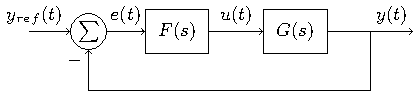
\includegraphics[width=0.6\linewidth]{../../figures/block1}
\end{center}
\end{frame}
\begin{frame}[label={sec:orga775da0}]{Feedback control}
\begin{center}
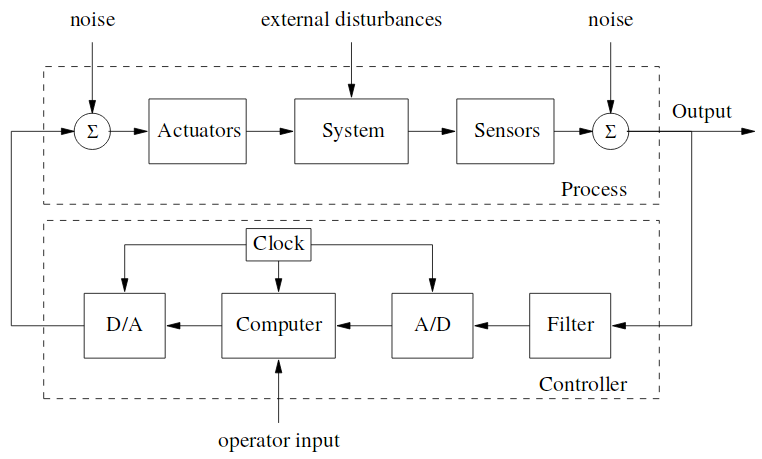
\includegraphics[width=0.7\linewidth]{../../figures/comp-contr-sys.png}
\end{center}
\end{frame}

\begin{frame}[label={sec:org60b1f50}]{Why computerized control?}
\end{frame}

\begin{frame}[label={sec:org194c76e}]{Computers everywhere}
\begin{center}
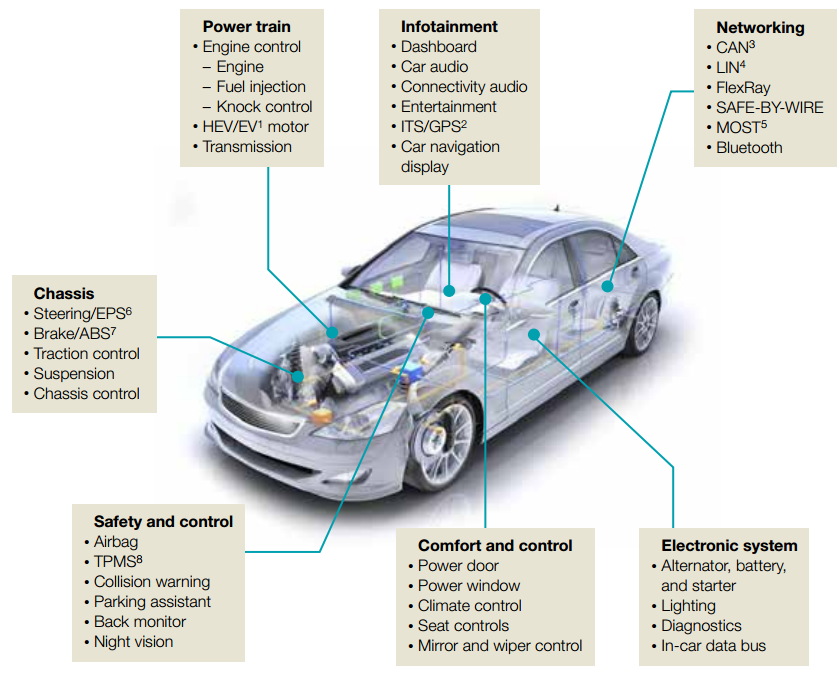
\includegraphics[width=0.7\linewidth]{../../figures/electronics-in-cars.png}
\end{center}
\begin{LaTeX}
\{\tiny Winning share in automotive semiconductors. McKinsey report 2013 \} 
\end{LaTeX}
\end{frame}

\begin{frame}[label={sec:org2716160}]{Two approaches to designing a  discrete-time controller}
\begin{enumerate}
\item Do design the controller in the continuous-time domain (methods from control engineering class). Then discretize the continuous-time controller.
\end{enumerate}
\pause
\begin{enumerate}
\item Determine discrete-time model of the plant. Do design in discrete-time domain.
\end{enumerate}
\end{frame}

\section{Discrete vs contionuous-time systems}
\label{sec:org11b8392}
\begin{frame}[label={sec:org024dd44}]{Discrete-time systems}
\[ x(k+1) = f\big(x(k),\, u(k)\big) \quad\Leftrightarrow\quad x_{k+1} = f(x_k,\, u_k)\]
\pause
Example:
\[ x_{k+1} = ax_k + bu_k \]
\pause
Introducing the shift operator \shift: \(\shift x(k) = x(k+1), \; \shift^{-1}x(k) = x(k-1)\)
\pause
\[ \shift x_k - ax_k = bu_k \quad\Leftrightarrow\quad (\shift - a)x_k = bu_k \quad\Leftrightarrow\quad x_k = \frac{b}{\shift-a} u_k. \]
\pause
Using the z-transform: \(\ztrf{x(k)} = X(z), \; \ztrf{x(k+1)} = zX(z) - x(0)\)
\pause
\[  zX(z) - x(0) - aX(z) = bU(z) \quad\Leftrightarrow\quad (z - a)X(z) = x(0) + bU(z)\]
\[ \quad\Leftrightarrow\quad X(z) = \frac{x(0)}{z-a}  + \frac{b}{z-a}U(z). \]
\end{frame}

\begin{frame}[label={sec:orgb90ee84}]{Exercise}
Consider the following discrete-time system

\begin{center}
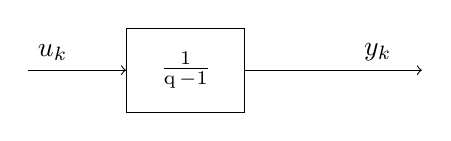
\begin{tikzpicture}[node distance=20mm,
                    block/.style={rectangle, draw, minimum width=15mm, inner sep=3mm},
                    sumnode/.style={circle, draw, inner sep=3pt}]
  \node[coordinate] (input) {};
   \node[block, right of=input,] (lti) {$\frac{1}{\shift -1}$};
   \node[coordinate, right of=lti, node distance=30mm] (output) {};
   \draw[->] (input) -- node[near start, above] {$u_k$}  (lti);
   \draw[->] (lti) -- node[coordinate] (meas) {} node[near end, above] {$y_k$} (output);
 \end{tikzpicture}
\end{center}

Recall the definition of the shift operator  \(\shift x(k) = x(k+1), \; \shift^{-1}x(k) = x(k-1)\).

\begin{enumerate}
\item Write the system as a difference equation \(y_{k+1} = f(y_{k}, u_k)\).
\item What is this type of system called?
\end{enumerate}
\end{frame}


\begin{frame}[label={sec:orgc4eba39}]{Homogenous solution}
\[ x(k+1) = a x(k), \quad x(0) = x_0 \]

\pause

\[ x(1) = ax(0) = ax_0\]

\pause

\[ x(2) = ax(1) = a^2x_0\]

\pause

\[ x(3) = ax(2) = a^3x_0\]

\pause
\[\vdots\]

\[ x(k) = a^k x_0\]
\end{frame}

\begin{frame}[label={sec:org1ecbc53}]{Homogenous solution to a first order system}
\[ x(k+1) = ax(k), \; x(0)=x_0 \quad\Rightarrow\quad x(k) = a^k x_0 \]

Pair each solution below to the corresponding value of \(a\) (\(x_0=1\)).
\[ \text{I)}\; a=1 \qquad \text{II)}\; a=2 \qquad \text{III)}\; a = 0.5 \qquad \text{IV)}\; a=-0.9 \]

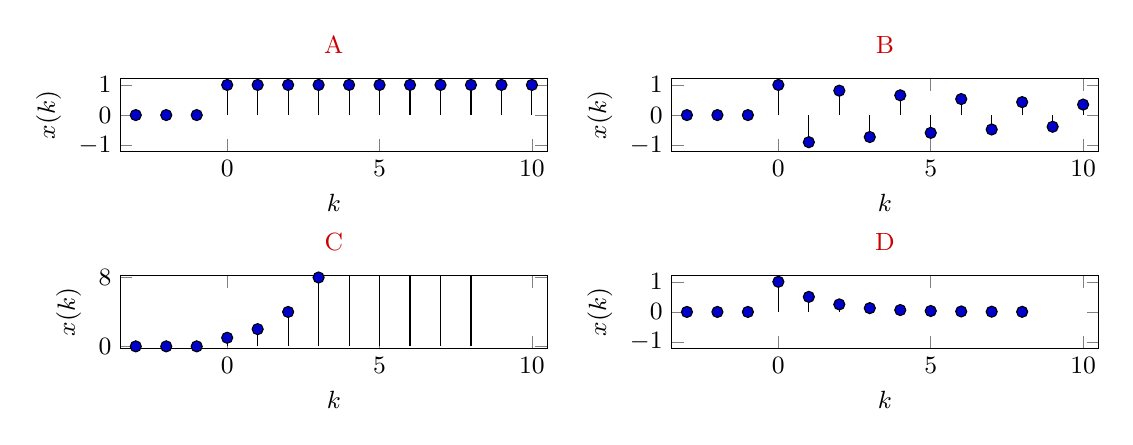
\begin{tikzpicture}
\small
\begin{axis}[
title={\textcolor{red!80!black}{A}},
width=7cm,
height=2.5cm,
xlabel={$k$},
ylabel={$x(k)$},
xmin=-3.5,
xmax=10.5,
ytick = {-1,0,1},
ymin = -1.2, ymax=1.2,
]
\addplot+[black, ycomb, domain=-3:10, samples=14,variable=k] { (k>=0)*pow(1,k)};
\end{axis}

\begin{axis}[
xshift=7cm,
width=7cm,
height=2.5cm,
title={\textcolor{red!80!black}{B}},
xlabel={$k$},
ylabel={$x(k)$},
xmin=-3.5,
xmax=10.5,
ytick = {0},
ytick = {-1,0,1},
ymin = -1.2, ymax=1.2,
]
\addplot+[black, ycomb, domain=-3:10, samples=14,variable=k] { (k>=0)*pow(-0.9,k)};
\end{axis}

\begin{axis}[
xshift=0cm,
yshift=-2.5cm,
width=7cm,
height=2.5cm,
title={\textcolor{red!80!black}{C}},
xlabel={$k$},
ylabel={$x(k)$},
xmin=-3.5,
xmax=10.5,
ytick = {0},
ytick = {-1,0,8},
ymin = -0.2, ymax=8.2,
]
\addplot+[black, ycomb, domain=-5:8, samples=14,variable=k] {  (k>=0)*pow(2,k) };
\end{axis}

\begin{axis}[
xshift=7cm,
yshift=-2.5cm,
width=7cm,
height=2.5cm,
title={\textcolor{red!80!black}{D}},
xlabel={$k$},
ylabel={$x(k)$},
xmin=-3.5,
xmax=10.5,
ytick = {0},
ytick = {-1,0,1},
ymin = -1.2, ymax=1.2,
]
\addplot+[black, ycomb, domain=-5:8, samples=14,variable=k] {  (k>=0)*pow(0.5,k)};
\end{axis}


\end{tikzpicture}
\end{frame}



\begin{frame}[label={sec:orgea16d5c}]{Discrete time vs continuous time}
\begin{center}
\begin{tabular}{l}
Continuous time\\
\hline
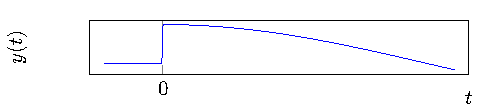
\includegraphics[width=0.4\linewidth]{../../figures/cont-fcn}\\
\(y(t)\)\\
\(\operatorname{p} y \triangleq \frac{d}{dt} y\)\\
\((\operatorname{p}+a) y = bu \;\Leftrightarrow\; \frac{d}{dt}y + ay = bu\)\\
\(Y(s) \triangleq \laplace{y(t)}\)\\
\(Y(s) = G(s)U(s) = \frac{b}{s+a}U(s)\)\\
Pole of the system: \(s+a=0 \; \Rightarrow \; s = -a\)\\
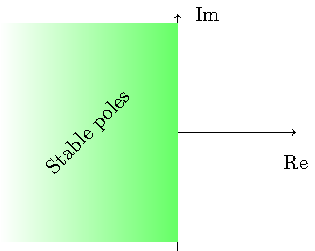
\includegraphics[width=0.22\linewidth]{../../figures/cont-stable}\\
\hline
\end{tabular}
\end{center}
\end{frame}

\begin{frame}[label={sec:org8f0d8ee}]{Discrete time vs continuous time}
\begin{center}
\begin{tabular}{ll}
Continuous time & Discrete time\\
\hline
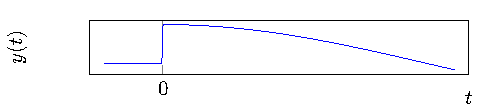
\includegraphics[width=0.4\linewidth]{../../figures/cont-fcn} & 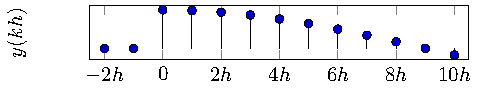
\includegraphics[width=0.4\linewidth]{../../figures/discrete-fcn}\\
\(y(t)\) & \(y(kh)\) or \(y(k)\)\\
\(\operatorname{p} y \triangleq \frac{d}{dt} y\) & \(\operatorname{q}y \triangleq y(kh+h)\)\\
\((\operatorname{p}+a) y = bu \;\Leftrightarrow\; \frac{d}{dt}y + ay = bu\) & \((\operatorname{q} + \alpha) y = \beta u \; \Leftrightarrow \; y(k+1) + \alpha y(k) = \beta u(k)\)\\
\(Y(s) \triangleq \laplace{y(t)}\) & \(Y(z) \triangleq \ztrf{y(kh)}\)\\
\(Y(s) = G(s)U(s) = \frac{b}{s+a}U(s)\) & \(Y(z) = H(z)U(z) = \frac{\beta}{z+\alpha}U(z)\)\\
Pole of the system: \(s+a=0 \; \Rightarrow \; s = -a\) & Pole of the system: \(z+\alpha = 0 \; \Rightarrow \; z = -\alpha\)\\
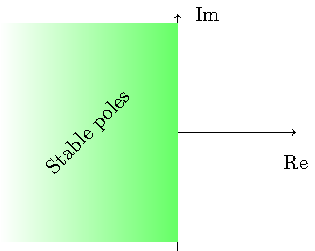
\includegraphics[width=0.22\linewidth]{../../figures/cont-stable} & 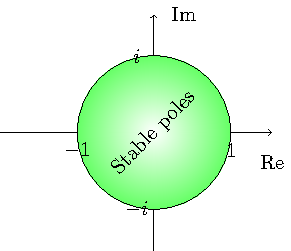
\includegraphics[width=0.22\linewidth]{../../figures/discrete-stable}\\
\hline
\end{tabular}
\end{center}
\end{frame}



\section{Further motivation for computerized control}
\label{sec:org700aa5e}
\begin{frame}[label={sec:org6e443a9}]{Discrete design can give better performance}
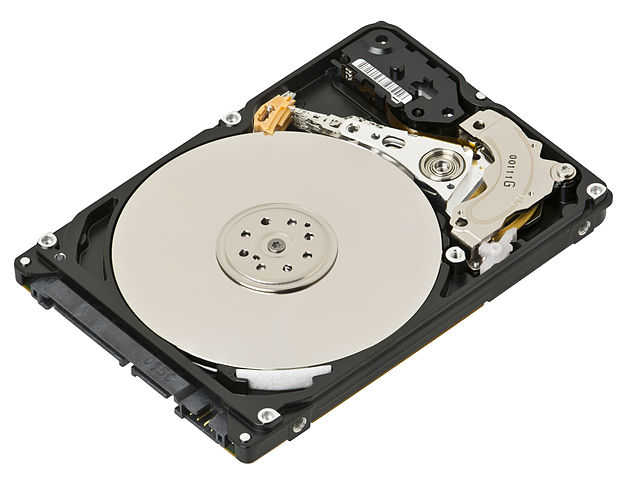
\includegraphics[height=0.5\textheight]{../../figures/diskdrive.png}
\end{frame}

\begin{frame}[label={sec:org4ab1a68}]{Discrete design can give better performance}
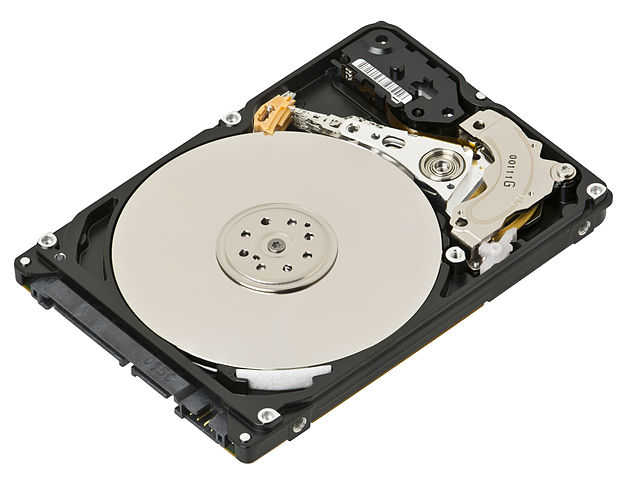
\includegraphics[height=0.5\textheight]{../../figures/diskdrive.png}
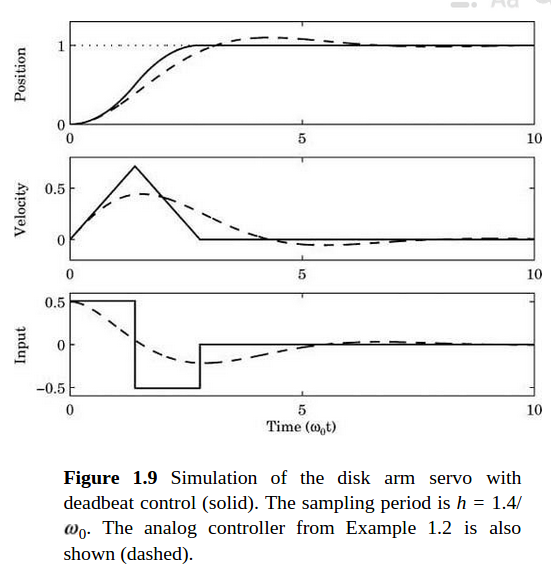
\includegraphics[height=0.8\textheight]{../../figures/fig1-9.png}
\end{frame}

\begin{frame}[label={sec:org9eaafb2}]{Challenges with computerized control}
\begin{block}{Aliasing}
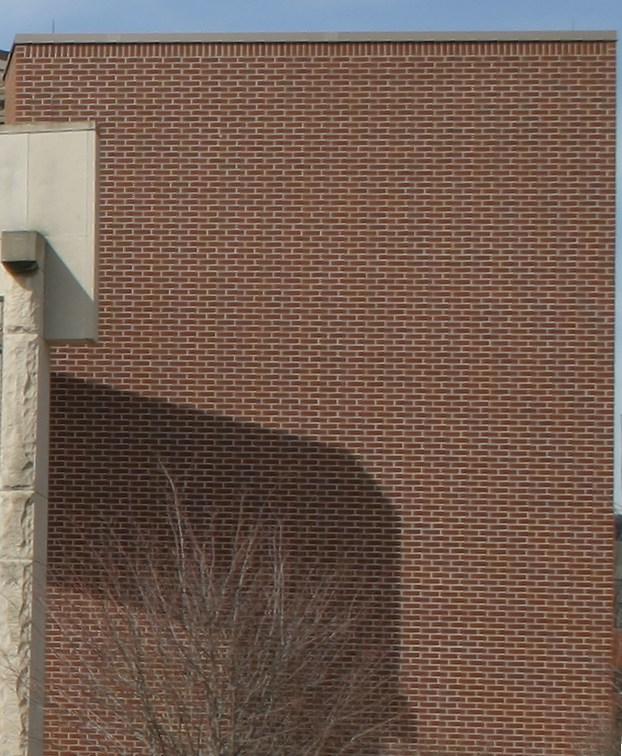
\includegraphics[height=0.6\textheight]{../../figures/Moire_pattern_of_bricks.png} \hspace*{3mm} 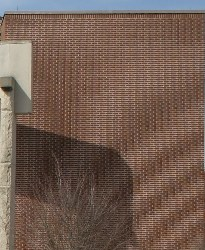
\includegraphics[height=0.6\textheight]{../../figures/Moire_pattern_of_bricks_small.png}
\end{block}
\end{frame}

\begin{frame}[label={sec:org2653894}]{Challenges with computerized control}
\begin{block}{Sampling causes delay}
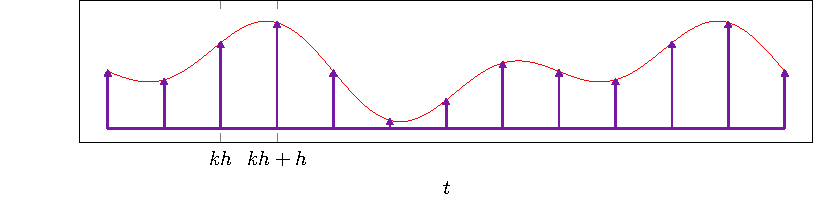
\includegraphics[width=0.9\textwidth]{../../figures/modulation-model-timeseries}
\end{block}
\end{frame}


\begin{frame}[label={sec:org7721946}]{Why learning computerized control?}
\begin{itemize}
\item Almost all control systems are implemented on computers/microcontrollers
\item Controllers designed in continuous-time must be discretized to be implemented on a computer - Performance can never be better than for continuous time.
\item Design that takes into account the discrete nature of the computer can give better performance
\end{itemize}
\end{frame}
\end{document}